%update: Jan 15 fixed grammar according to prof notes
%update: Jan 13 prof rewrite for ithenticate
%update: Jan 09-11 prof check
%update: Jan 07 rephrased all. add table 5.1
%update: Dec 20 ref done
%update: Dec 13 figures added
%update: Nov 21 first copy draft

%\begin{savequote}[75mm] 
%You may say I'm a dreamer, but I'm not the only one. I hope someday you'll join us. And the world will live as one.
%\qauthor{John Lennon} 
%\end{savequote}

\chapter{Opto-Mechano-Electrical Tripling in Zinc Oxide Nanowires Probed by \emph{In situ} Photocurrent Spectroscopy in TEM}

\newthought{For future flexible optoelectronics}, three important factors must be considered: light, force and electricity. 
Thus, photosensing spectroscopy of free-standing Zinc Oxide (ZnO) nanowires in a high-resolution transmission electron microscope (TEM) is studied herein. 
By applying the optical {\em in situ} TEM system described in Chapter 2, novel opto-mechano-electrical tripling phenomenon in Zinc Oxide nanowires is discovered. 
Interestingly, splitting of photocurrent spectra at ~3.3 eV under {\em in situ} TEM bending of Zinc Oxide nanowires directly corresponds to the nanowire deformation. It is established that such effect is caused by the expanded and compressed nanowire sides, especially at the nanowire edges. 
Theoretical calculations of deformed Zinc Oxide nanowire bend structure changes has a perfect agreement with the {\em in situ} experimental data. 
The splitting of photocurrent spectra can be understood in terms of changes in the valence band structure of Zinc Oxide nanowires because of the lattice strain. 
The deformation-induced splitting gives a valuable information for flexible optoelectronics and piezo-phototronics when using nanowire building blocks. 

\section{Introduction}

These years, transmitting information at a wide band width, long distance, ultra-high speed and low power consumption relies on photons passing through optical fibers, instead of using electrons in electrical wires. 

However, the industries and consumers are still not satisfied with the current status of integrations of optoelectronic components within rigid or flexible substrates.\cite{C.2009, T.2004, D.2004}
To achieve highly efficient integrations with multi-functionalities, the sizes of light sources (including laser diodes and light emitting diodes), modulators, resonators, waveguides, photodetectors in optoelectronic systems or even additional strain sensors, accelerometers etc. in Micro-Opto-Electro-Mechanical Systems are expected to be downsized to the nanoscale.\cite{Park2007} 
To catch up with the currently mature silicon microelectronics industries, the light-matter interactions in novel optoelectronic semiconducting materials should be carefully studied, especially with respect to using them as individual building blocks for bottom-up optoelectronic technology. 
However, conventional approaches are not able to detect, operate and modify optoelectronic property/functions of a single nanomaterial directly and at the high spatial resolution. 

\begin{figure}  
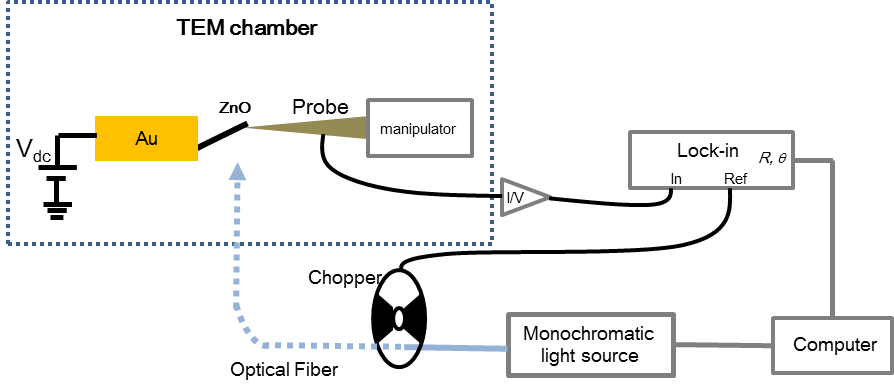
\includegraphics[width=\textwidth]{figures/figure5_1}
\caption[Experimental setup for Zinc Oxide.]{Scheme of experimental setup for the ZnO nanowire inside and outside of a high-resolution TEM.
\label{fig:5_1}}
\end{figure}

In addition, flexible and stretchable electronics and optoelectronics attract prime attention of general consumers nowadays. 
Nanowires, as one of the most promising building blocks for bottom-up flexible optoelectronics, have not been yet comprehensively studied at a level of a single free-standing material. 
A zinc oxide nanowire is one of the most promising and hot 1-D materials for opto-mechano-electrical applications because of its ideal piezo-phototronic properties.\cite{L.2011a,L.2010,Xu2015b,L.2010a} 
Many published reports on flexible nanowire photodetectors have relied on various substrates.\cite{G.2015,H.2014,G.2014} 
Obviously, choosing a right substrate is always an essential factor in flexible optoelectronics; that is, the physical properties of a nanostructure are strongly affected by the substrates. 
For instance, it has been reported that the optical absorption coefficient, the band-edge and near-band-edge (NBE) characteristics of zinc oxide films are very much dependent on the substrate type/quality and its treatments.\cite{R.1997} 
Consequently it is very important to characterize mechano-optoelectronic properties of zinc oxide nanostructures in free-standing conditions and in high vacuum. 
For example, Ohno et al. studied photoluminescence (PL) and cathodoluminescence (CL) spectra of a piece of the diamond crystal in TEM;\cite{S.1995} 
Yang et al. measured photocurrent values of deformed zinc oxide nanowires in TEM after their illumination by light with fixed wavelength.\cite{E.2012} 
However, the wide-band-range photocurrent spectroscopy of free-standing zinc oxide nanowires or any other nanomaterials has not been researched as yet. 
In this Chapter, I investigate the photocurrent spectroscopy of individual free-standing zinc oxide nanowires by means of {\em in situ} probing optical-STM-TEM. 
It is discovered that the photocurrent spectra of zinc oxide nanowires experience a specific splitting. Additionally, the splitting values exactly correlate with the elastic strains applied. 
Under relevant theoretical calculations, the valence band structure is found to change accordingly on two sides of the bent nanowire. The calculations nicely fitted and matched the experimental results. 

\section{Experimental}

Zinc oxide nanowires were prepared through a chemical vapor deposition (CVD) method similar to that in previous reported publications.\cite{Xu2015b}
{\em In situ} characterizations and manipulations were performed by the optimized {\em Nanofactory Instruments AB} opto-TEM-STM sample holder with a nanomanipulator and an optical fiber, as detailed in Chapter 2, in a 300 kV JEOL-3100FEF (Omega filter) high-resolution microscope. 
Zinc oxide nanowires were carefully placed onto the gold wire stage of the holder tip-frame by using the minimum amount of silver epoxy. 
Then, inside TEM, the electrochemically etched tungsten probe was moved to contact a chosen individual nanowire by controlling the piezo-nanomanipulator movements. Also, the optical fiber was manipulated to illuminate the specimen in tandem with its probing. 
The experimental configuration is schematically shown in Figure \ref{fig:5_1}. 
By controlling the tungsten probe, deformation of nanowires was delicately carried out. 
The photocurrent was then tested by applying a voltage between the two ends of a zinc oxide nanowire. While, with the aid of the monochromator, scanning of the light wavelength from 2.5 eV to 4.5 eV, and recording the photocurrent spectrum were performed. 
By applying a lock-in amplifier, photocurrent response was rectified according to the chopper frequency in order to resolve the weak signals from the noise background. 
\vfill % gap

\begin{figure}  
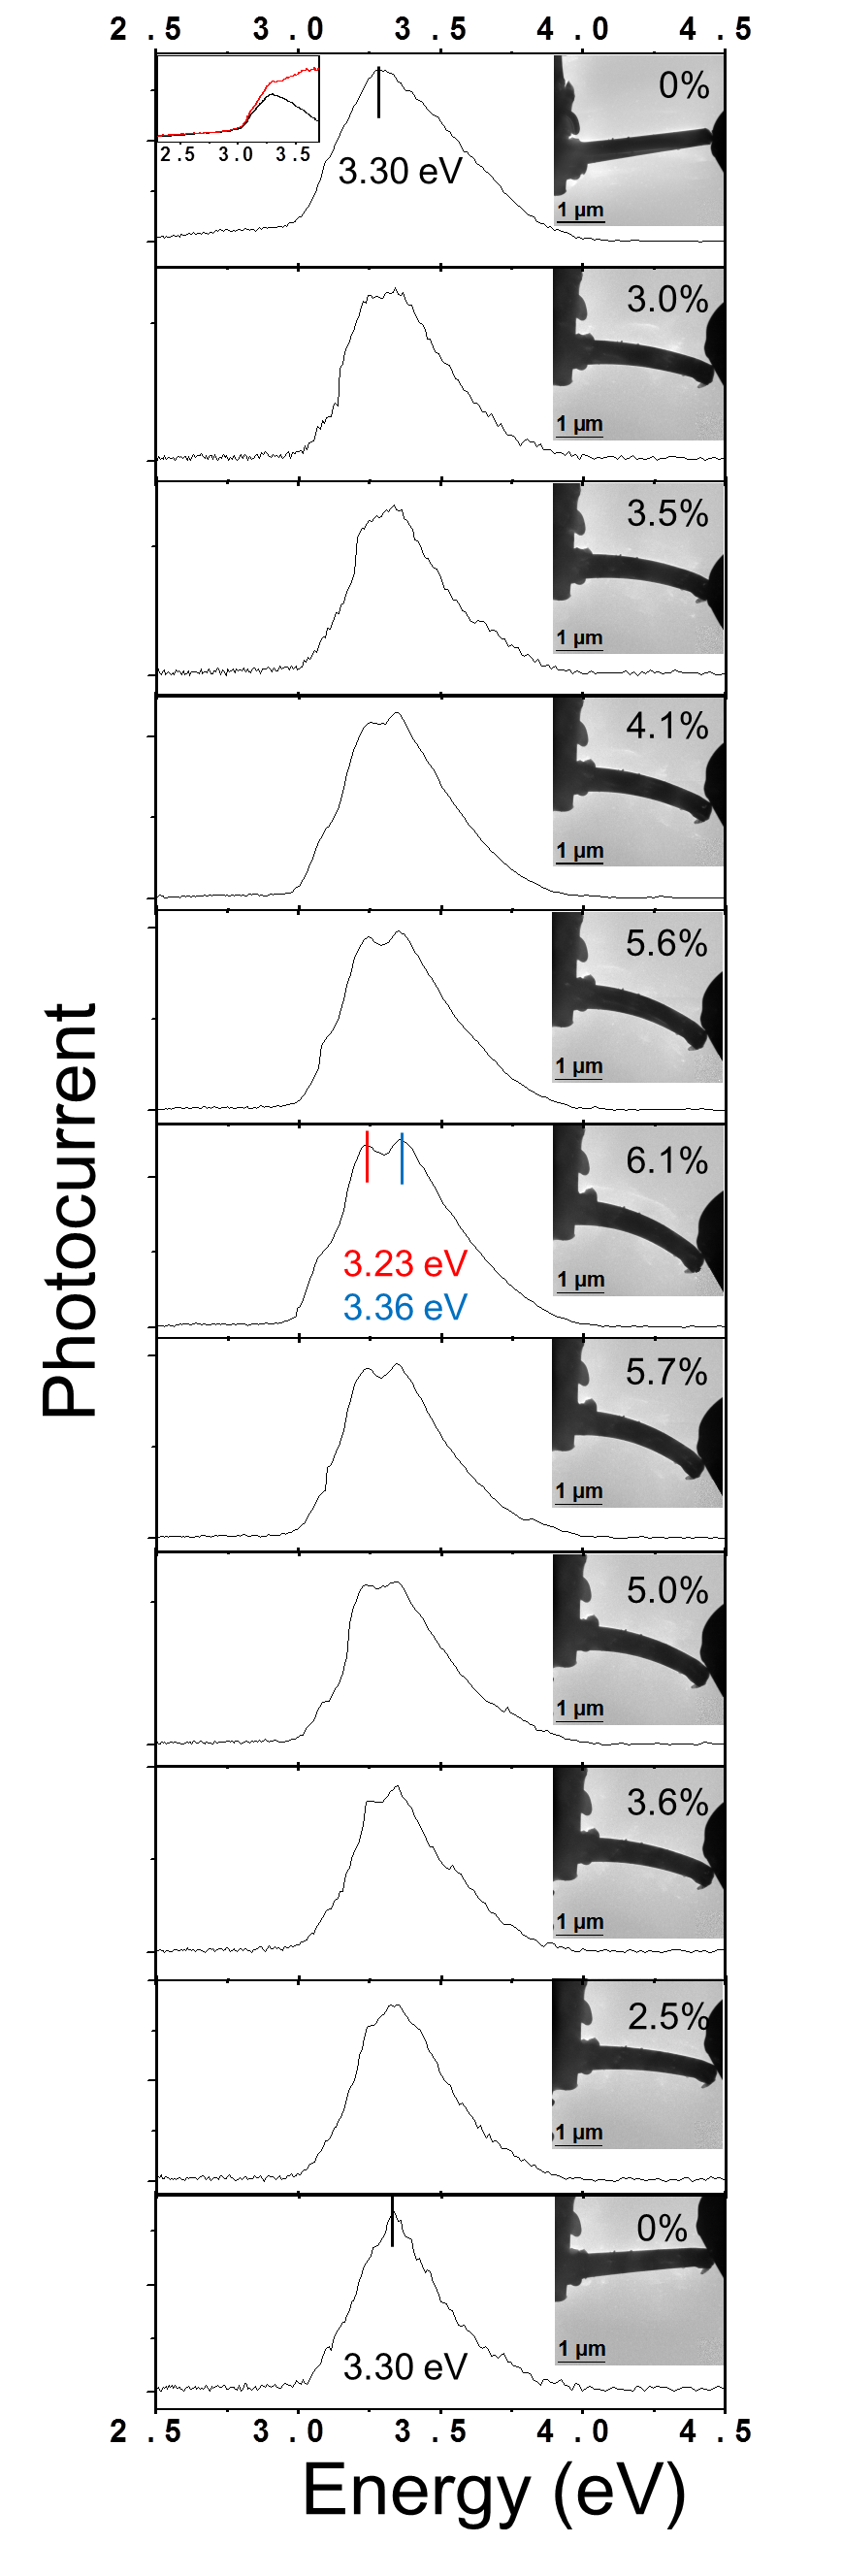
\includegraphics[width=191pt]{figures/figure5_2}
\centering
\caption[Splitting of photocurrent spectra]{Photocurrent spectra (raw data) recorded under bending deformations from 0\% to 6.1\%, and back to 0\%. Red line in the upper left inset of the first panel depicts the normalized (to the incident photons) spectrum at a zero strain (normalized from the measured photocurrents shown as the black line in the inset).
\label{fig:5_2}}
\end{figure}

\section{Results and discussions}

In Figure \ref{fig:5_2}, an experimental run on a given zinc oxide nanowire is shown. The nanowire was initially straight, as illustrated in the uppermost panel of Figure \ref{fig:5_2}. 
Please note that the normalized spectrum to the incident photons at the zero strain state was calculated and is shown in the inset. 
Due to the large exciton binding energy at ~60 meV for ZnO, a strong exciton absorption peak is seen even at room temperature. 
The nanowire was probed under its bending in the horizontal plane. 
Photocurrent-wavelength raw spectra in Figure \ref{fig:5_2} demonstrate the specific splitting phenomenon which is apparently related to the strain in the deformed nanowire. 
The nanowire diameter was measured to be ~385 nm. 
The strain, was calculated as follows \footnote{Please note that the strain value determination is intrinsically the same as that in  Chapter 6 but with  2 times constant difference }: $$\epsilon = \frac{r}{R} $$
, where $r$ is a distance from the compressed or expanded side of the nanowire to the middle point of the compressed or expanded region and $R$ is the radius of curvature of the deformed nanowire. \\

The first manipulation deformed the nanowire to 3.0\% strain and then to 3.5\%, 4.1\%, 5.55\% and 6.1\% gradually. 
Next, the probe was carefully moved backwards. 
The strains then decreased to 5.66\%, 5.0\%, 3.6\% and 2.5\% gradually. 
Finally, the nanowire returned to its original unbent state. 
Before taking any photocurrent spectrum after each probing, the electron beam of the microscope was taken off and away from the sample. 
One side of the deformed nanowire experiences a compressive strain; the other side is under tension. 
The high-resolution TEM image, as shown in Figure \ref{fig:5_s2}, clearly displays the (002) lattice fringes along the c-axis, which is also the growth direction of the nanowire.\cite{zhang2015opto} 
The local lattice distance within the compressed nanowire edge is ~0.243 nm, which is smaller than the usual value of 0.260 nm of the ZnO bulk material.\cite{L.2011} 
The local lattice distance is larger away from the compressed edge, up to 0.257 nm. 
Once the nanowire is bent, at first, the photocurrent spectra remain a of very similar shape displaying one broad peak centered at about 3.30 eV. 
Once the strain is increased under further \textit{in situ} bending, the pristine broad peak splits into two components. 
Upon a 3.0\% strain, the separated two peaks are centered at 3.24 eV and 3.34 eV. 
Therefore the corresponding red-shift and blue-shift are 0.06 eV and 0.04 eV, respectively. 
Upon the largest strain applied at 6.1\%, the red-shift becomes larger, about 0.07 eV, while the blue shift is 0.06 eV. 
The splitting values are determined by the gap between the centers of the two peaks of the photocurrent spectra on the deformed nanowire. These are listed in sequence in Table \ref{tab:5_1}. 
\begin{table}
    \centering
    \begin{tabular}{c|c}
    \hline
         Splitting Values (eV) & Strain\\
         \hline
         0.01 & 3.0\%\\ 
         0.09 & 3.5\%\\
         0.10 & 4.1\%\\
         0.12 & 5.6\%\\
         0.13 & 6.1\%\\
         0.11 & 5.7\%\\
         0.13 & 5.0\%\\
         0.10 & 3.6\%\\
         0.08 & 2.5\%\\
         \hline
    \end{tabular}
    \caption{Splitting values of photocurrent spectra on the deformed nanowire}
    \label{tab:5_1}
\end{table}
 
The peak positions are also plotted in Figure \ref{fig:5_3}d to clearly depict the relationship. 
It is clear that there is an obvious correlation between the strain and the peak position shifts. 
To get the deeper insights into such correlation, the theoretical calculations were conducted. 

Photocurrent spectroscopy is one of the most important methods to obtain the band gap information from crystals. 
So, researchers have typically explained photocurrent behaviors in the frame of band gap theories. 
In my work, zinc oxide nanowire is appeared to be a highly crystalline direct band gap material tested without a substrate and in high vacuum. During bending, no other variables are added. 
Under such ideal conditions, it is reasonable to assume that changing of the band gap is directly correlated with the energy values of the photocurrent peak and its splitting. 
The total spectra containing an overall photoresponse might be mainly affected by the surface of the nanowire rather than its total body, also they may be affected by some pre-existing defects (usually oxygen vacancies, not created by bending), hence, the spectrum broadening due to splitting is probably hidden. 
Another detail is that the fiber transmission efficiency in my experiment is somewhat limited. 
The transmission efficiency decreases quite a lot at the UV range, at around 400 nm (or 3.1 eV), which cuts off the intensity of the incident light energy. 

\begin{figure}  
\centering
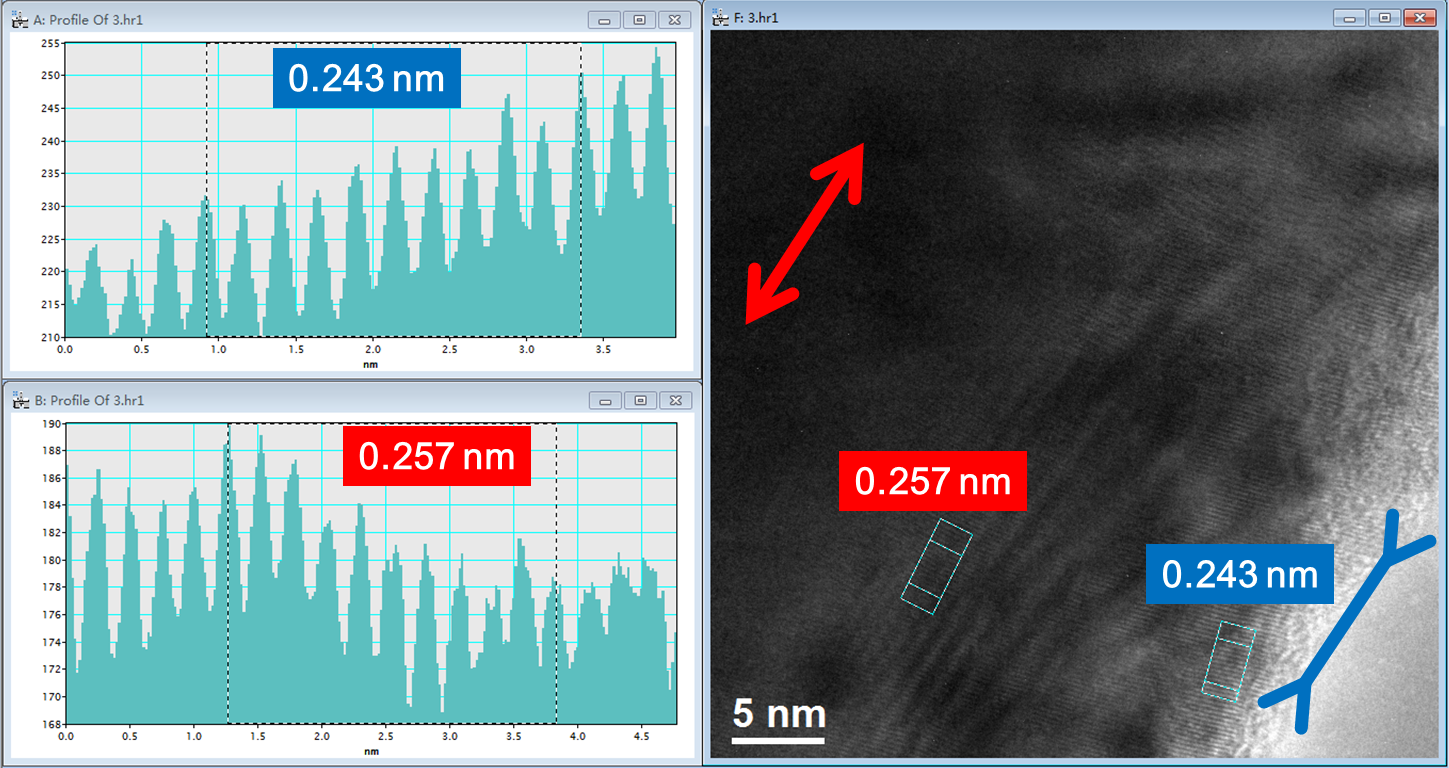
\includegraphics[width=\textwidth]{figures/figure5_s2}
\caption[Localized strain in HRTEM image]{High-resolution TEM image of a deformed Zinc Oxide nanowire. The (002) lattice fringe separation is 0.243 nm at the most compressed sample edge, and 0.257 nm at the less compressed core. 
\label{fig:5_s2}}
\end{figure}


Theoretical calculations for deformed ZnO nanowires were performed by using Density Functional Tight Binding (DFTB) method which is implemented in the DFTB+ software package.\cite{T.2007} 
DFTB approach has widely been used for the accurate and efficient description of electronic, structural and transport properties of various inorganic materials especially for those which contain more than 1000 atoms in the simulation system. 
However, we are still limited by the simulation capability with regard to the number of atoms involved. 
Therefore we chose to simulate a ZnO nanowire with a diameter of 1.5 nm. 
Parametrization of Zn atom interactions with O atoms has been used for various bulk Zn-crystals such as hcp-Zn, zinc-blende-ZnS and wurtzite-Zinc Oxide, and ZnO surfaces (surface is clean with a small amount of adsorbates), and Zinc Oxide nanostructures. 
Such parameterization provided a good description of electronic band structures of zinc oxide including reasonable representations of the band structure and its band gap of 4.1 eV.\cite{Moreira2009}

\begin{figure}  [ht]
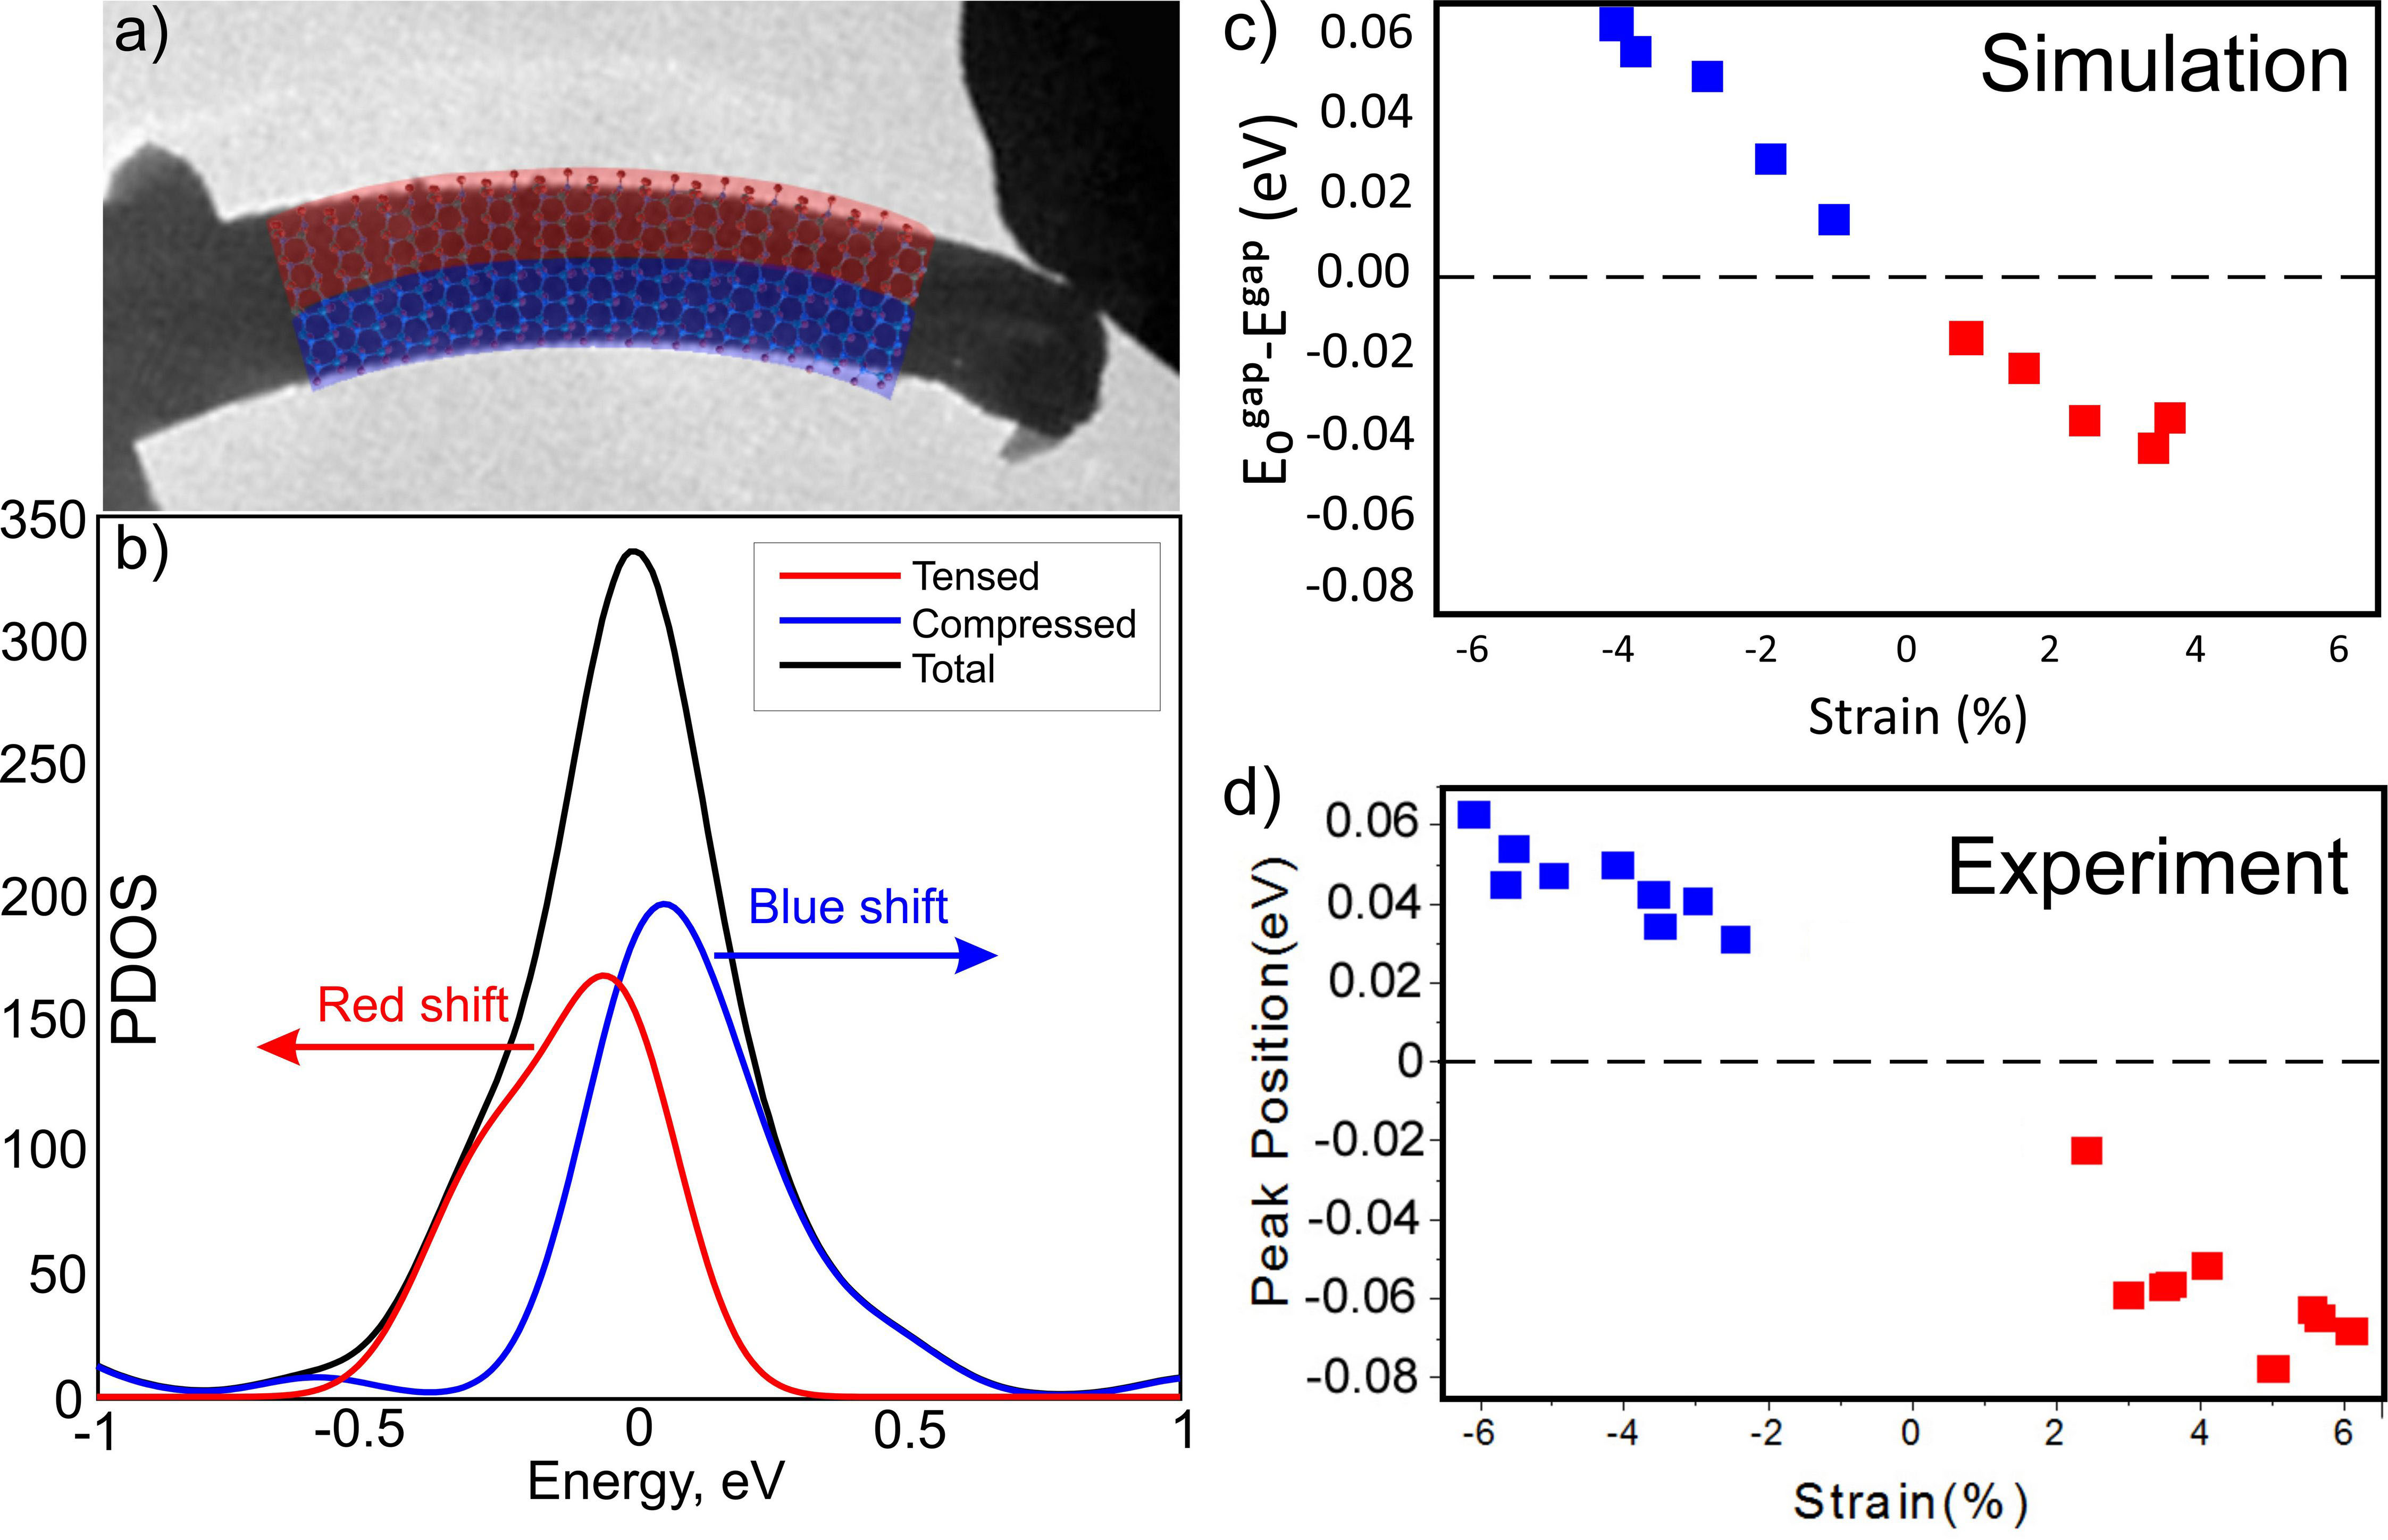
\includegraphics[width=\textwidth]{figures/figure5_3}
\caption[DFTB calculations match experimental results]{(a) Computed geometry of a deformed Zinc Oxide nanowire in accord with the experimental data. The simulated structure is divided into two domains (marked by red and blue colored portions) for the simulation of PDOS in expanded and compressed regions. Notice that the size of calculated geometry is not the same as for the experimental picture. (b) PDOS of expanded (red) and compressed (blue) sides of the deformed Zinc Oxide nanowire. Black curve shows the total DOS for the unbent nanowire, as a whole. Bending strain is ~4\%. (c) Dependence of the Zinc Oxide wire band gap on the bending strain in the frame of the DFTB approach adopted; (d) Dependence of the photocurrent peak position on the bending strain obtained experimentally. Red and blue colors denote the expanded and compressed regions of Zinc Oxide nanowires, respectively. 
\label{fig:5_3}}
\end{figure}


We simulated a bent zinc oxide nanowire with various degrees of curvature and in accordance with the experimental deformation values, as shown in Figure \ref{fig:5_3}a.
Two sides of the nanowire are marked by red or blue colors along with its expanded or compressed portions, respectively. \\
A simulated zinc oxide nanowire is constructed by 1500 atoms of Zn and O. 
To exclude the effect of dangling bonds and surface currents on the deformed structures, the simulated supercell surface was covered by a uniform layer of hydrogen atoms. 
Splitting of the photocurrent spectra is directly related to the splitting of levels in the valence band at $\Gamma$ point with the corresponding red/blue shifts of the peaked wavelength values under bending. .\cite{Liao2012} \\
The values of splitting partial density of states (PDOS) were calculated for the expanded and compressed sides of a nanowire, as shown in Figure \ref{fig:5_3}b. 
During bending under TEM probing, the position of the conduction band was not changed. 
Only the valence band was affected. \\
In Figure \ref{fig:5_3}b, the alternations in the valence band of the bent zinc oxide nanowire experiencing a strain of ~4\% are shown. 
PDOS peculiar to the expanded/compressed sides of the zinc oxide nanowire are marked in red and blue colors, respectively. 
Calculation results imply that the valence band shifts in a direction of a red range of wavelengths, whereas the compression causes the blue shift. 
This is a perfect match with the experimental data. \\
More simulations were also carried out for zinc oxide nanowires having various bending deformations from 1\% to 4\%. 
As shown in Figure \ref{fig:5_3}c, these reveal a clear dependence of the band gap on strain.  
The changes of the band gap are obviously correlated with the changes in the photocurrent peak center, as measured in the {\em in situ} probing experiments, Figure \ref{fig:5_3}d. 
Thus the obtained computational data exhibit a perfect agreement with the experimental data. \\

A few published results on deformed zinc oxide nanowires or microwires are in consistence with ours. 
For example, Xue et al. studied the strain effects on NBE of ZnO, which are characterized by CL inside a scanning electron microscope (SEM). They found that the emissions had had a relation with the strain.\cite{G.2010}
Liao et al. also researched CL splitting and shift in deformed zinc oxide microwires in SEM. It is noted that the relationship between the excitation spectra evolution and compressive edges was rather clear. Also, it is believed that the valence band splitting would contribute to the NBE splitting.\cite{Moreira2009} 
In my {\em in situ} probing experiments, the splitting takes place not during CL measurements (a process stimulated by electron beam to emit light) but during recording of a photoresponse as the electrical current. 
This is a result of light absorption and the generation of electron-hole pairs.
But, anyway, both processes share the same strain conditions that result in splitting of energy levels in the valence band at the Г point. 

\section{Conclusions}
To conclude, this Chapter discussed on opto-mechano-electrical tripling phenomena under {\em in situ} imaging and probing measurements of photocurrents in zinc oxide nanowires in real time, and under high spatial resolution. 
By comparing photocurrent spectra of individual free-standing zinc oxide nanowires under strain, splitting of photocurrent spectra was recorded. 
The shifts of photocurrent peaks were in an obvious correlation with the bending strains. 
The red/blue shifts were proved to be directly related to the splitting of energy levels in the valence band at the $\Gamma$ point. 
DFTB calculations documented a perfect match with the {\em in situ} experimental results. 
The splitting of photocurrent spectroscopy gives an important clue for future flexible optoelectronics and piezo-phototronics. 
For example, it would be highly useful for strain-tuned wavelength-division multiplexing modules or MOEMS devices, and for flexible optoelectronics where photocurrent splitting values must be evaded as a key variable. 